\documentclass{beamer}
 
\usepackage[utf8]{inputenc}
 
\usetheme{Madrid}
\setbeamertemplate{theorems}[numbered]
 
 
\begin{document}

%Information to be included in the title page:
\title[BSD]{Verifying some consequences of the \\ Birch Swinnerton-Dyer Conjecture}
\author[Felipe Jacob]{\begin{tabular}{r@{ }l}
                        Author: & Felipe Jacob \\
                        Supervisor: &Dr Richard Hill
                                      \end{tabular}}
\institute[UCL]{University College London}
\date{March 22, 2017}

\newcommand{\defin}{\textbf}
\newcommand{\CC}{{\mathbb C}}
\newcommand{\cov}{{\operatorname{cov}}}
\newcommand{\eE}{{\mathcal E}}
\newcommand{\NN}{{\mathbb N}}
\newcommand{\PP}{{\mathbb P}}
\newcommand{\ZZ}{{\mathbb Z}}
\renewcommand{\SS}{{\mathbb S}}
\newcommand{\DD}{{\mathbb D}}
\newcommand{\RR}{{\mathbb R}}
\newcommand{\QQ}{{\mathbb Q}}
\newcommand{\rR}{{\mathcal R}}
\newcommand{\OO}{{\mathcal O}}
\newcommand{\p}{\partial}
\newcommand{\mM}{{\mathcal M}}
\newcommand{\pP}{{\mathcal P}}
\newcommand{\iI}{{\mathcal I}}
\newcommand{\jJ}{{\mathcal J}}
\newcommand{\uU}{{\mathcal U}}
\newcommand{\sS}{{\mathfrak S}}
\newcommand{\1}{{\mathds 1}}
\newcommand{\Crit}{\operatorname{Crit}}
\newcommand{\GKK}{{G_{\bar{K} : K}}}
\newcommand{\st}{{\text{s.t.}}}
\newcommand{\ra}{\rightarrow}
\newcommand{\Sel}{\text{\normalfont Sel}}
\newcommand{\Sha}{\text{\normalfont Sha}}
\newcommand{\TS}{\text{\normalfont TS}}
\newcommand{\Eb}{\bar{E}}
\newcommand{\EQ}{E(\QQ)}
\newcommand{\cmark}{\textrm{\ding{51}}}
\newcommand{\xmark}{\textrm{\ding{55}}}
\newcommand{\EFp}{{\tilde{E}(\FF_p)}}
\newcommand{\EFt}{{\tilde{E}(\FF_2)}}
\newcommand{\EQp}{{E(\QQ_p)}}
\newcommand{\FF}{\mathbb{F}}
\newcommand{\HH}{\mathbb{H}}
\newcommand{\Tors}{{\text{\normalfont Tors}}}
\newcommand{\parder}[2]{\frac{\partial #1}{\partial #2}}
\newcommand{\Zpx}{\mathbb{Z}_p^\times}
\newcommand{\legendre}[2]{\left(\frac{#1}{#2}\right)}
\newcommand{\quadring}[1]{\ZZ[\sqrt{#1}]}
\newcommand{\Ip}{\mathfrak{p}}
\newcommand{\Aa}{\mathbb{A}}
\newcommand{\LL}{\mathcal{L}}
\newcommand{\Shim}{\textnormal{Shim}}

\frame{\titlepage}
 
\begin{frame}
\frametitle{Elliptic Curves}
An \textbf{Elliptic Curve over a field $K$} is a projective variety $E$
where
\begin{itemize}
\item $E$ is a cubic curve over $\PP^2(K)$
\item $E$ is nonsingular over $K$
\item There exists a distinguished $\OO \in E(K)$ called the \textbf{point at infinity}.
\end{itemize} \pause
\bigskip

\textbf{Example}: $E: y^2z = x^3 - xz^2$ is an elliptic curve over
$\QQ$ with $\OO = (0:1:0)$
\end{frame}

\begin{frame}
\frametitle{Elliptic Curves}
  If $\text{char}(K) \neq 2$, we can assume $E$ has the affine model
  \[y^2 = x^3 + ax^2 + bx + c,\]
  with $a, b, c \in K$, and $\OO = (0:1:0).$
\end{frame}

\begin{frame}
  \frametitle{Group Law}
  Actually, $E(K)$ has a natural addition law.
  \bigskip

  To add two distinct points $P, Q$, we trace the line
  between them and let $R$ be the third point of intersection of this line with
  the curve. $P+Q$ is then the reflection of $R$ over the $x$-axis. \pause
  \begin{figure}
    \centering
  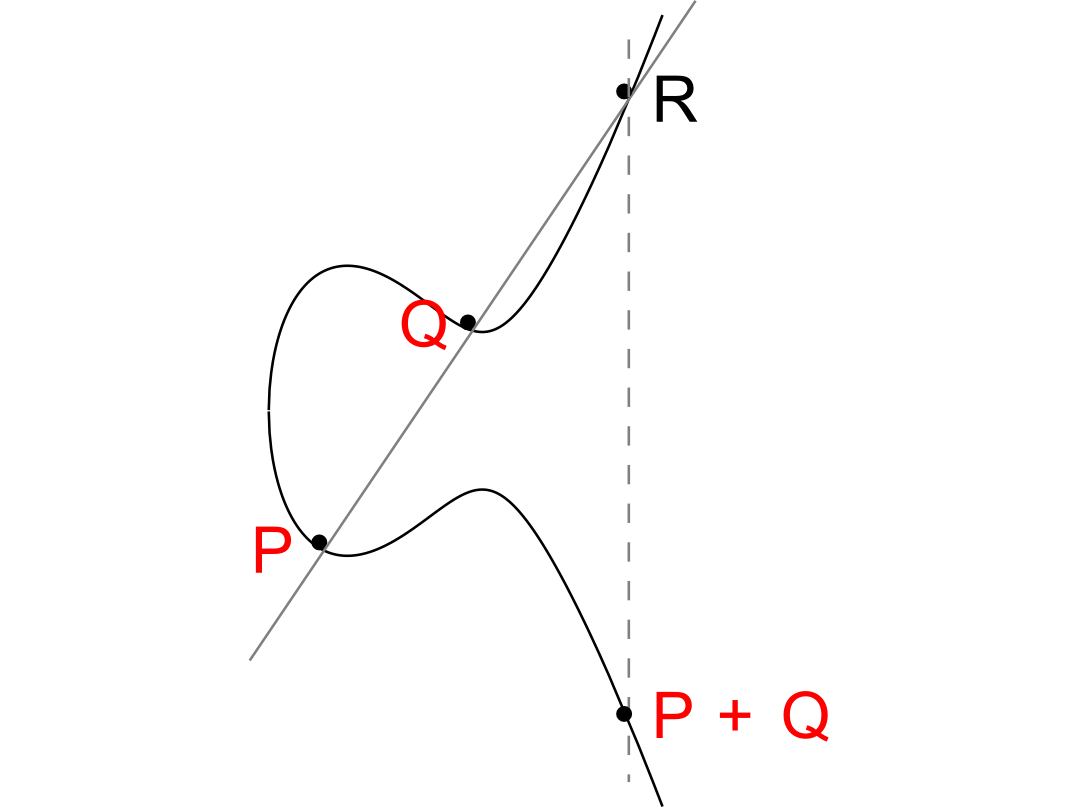
\includegraphics{picture3}
  \end{figure} \pause

  Under the operation $+$, it turns out $E(K)$ is an abelian group, with $0 = \OO$.
\end{frame}

\begin{frame}
  \frametitle{Quadratic Twists}
  The curves we will be interested in this project are given by
  \[E_n : y^2 = x^3 - n^2 x,\]
  where $n$ is odd and squarefree. \pause

  They are notorious for their relation with Fermat, Gauss and the
  congruent number problem.
\end{frame}

\begin{frame}
  \frametitle{The Rank I}
  \begin{theorem}[Mordell-Weil]
    Let $E$ be an elliptic curve over $\QQ$. Then $E(\QQ)$ is finitely generated.
  \end{theorem} \pause

  This means we can write
  \[E(\QQ) = \Tors(E(\QQ)) \times \ZZ^r\]
  where
  \begin{itemize}
  \item $\Tors(E(\QQ))$ is finite.
  \item $r$ is a natural number called the \textbf{rank of $E$}.
  \end{itemize}
\end{frame}

\begin{frame}
  \frametitle{The Rank II}
  \begin{theorem}
    Our curves
    \[E_n : y^2 = x^3 - n^2 x\]
    have 4 points of finite order: $\Tors(E(\QQ)) = \{\OO, (0,0), (n, 0), (-n,0)\}.$
  \end{theorem} \pause
  \bigskip

  Finding $r$, however, is \textbf{hard}.
  
\end{frame}
 
\begin{frame}
  \frametitle{The BSD Conjecture}
  The Birch Swinnerton-Dyer Conjecture relates the rank $r$ of an elliptic
  curve $E$ to the order of a zero of a certain analytic function. \pause

  More precisely, it says that
  \[L(E,s) = C (s-1)^r + O((s-1)^{r+1}),\]
  where $L(E,s)$ is an analytic function called the \textbf{Hasse-Weil
    L-function of $E$}. We will see how to construct it.
\end{frame}
 
\begin{frame}
  \frametitle{Local Zeta Functions I}
  Let $p$ be a prime number.
  If $V$ is a variety over $\FF_p$, we can construct the \textbf{Local Zeta
    Functions of $V$ at $p$}, given by
  \[Z(v,p,z) = \prod\limits_{M \triangleleft C_E} \frac{1}{1 - ||M||^{-z}}\]
  where $M$ are the maximal ideals of $C_E := \frac{\FF_p[x,y]}{E}$ 
  
\end{frame}

\begin{frame}
  \frametitle{Local Zeta Functions II}
  We also have the computational formula
  \[Z(V,p,s) = \exp \left( \sum\limits_{k=1}^\infty \# V(\FF_{p^k})
      \frac{z^k}{k} \right),\] 
  so we get $Z$ from knowing how many points $E$ has in at every finite field of
  $p^k$ elements.
\end{frame}

\begin{frame}
  \frametitle{Local Zeta Functions III}
  \textbf{Example:} If $V = (x_0,y_0)$ is a point, then $\# V(\FF_{p^k}) = 1$, so we get
  \begin{equation*}
    \begin{split}
      Z(V,p,s) &= \exp \left( \sum\limits_{k=1}^\infty \frac{z^k}{k} \right)
      = \exp \left( -\log (1-z) \right) \\
      &= \frac{1}{1-z}
    \end{split}
  \end{equation*} \pause

  \textbf{Example:} $V = \PP^n$, we know that $\# V(\FF_{p^k}) = 1 + p^k + \cdots +
  p^{nk}$, so we get 
  \[Z(V,p,z) = \frac{1}{1-z} \frac{1}{1-pz}\cdots \frac{1}{1-p^nz}\]
\end{frame} 

\begin{frame}
  \frametitle{Hasse-Weil Zeta Function I}
  To form the \textbf{Hasse-Weil L-function of $V$},
  we multiply the local zeta functions
  of $V$ for all different primes:

  \[\zeta(V,s) = \prod\limits_p Z(V,p,p^{-s}).\] 

  This function captures the behaviour of $V$ at all possible finite fields.

\end{frame}

\begin{frame}
  \frametitle{Hasse-Weil Zeta Function II}
  \textbf{Example:} If $V$ is a point, we get
  \[\zeta(V,s) = \prod \limits_p \frac{1}{1-p^{-s}} = \zeta(s),\]
  which is the standard Riemann-Zeta function. \pause
  \bigskip

  \textbf{Example:} If $V = \PP^n$ we instead get
  \[\zeta(V,s) = \zeta(s) \zeta(s-1) \cdots \zeta (s-n).\]
\end{frame}

\begin{frame}
  \frametitle{Hasse-Weil Zeta Function III}

  \begin{theorem}
    For the curves
    \[E_n : y^2 = x^3 - n^2 x,\]
    with $n$ is odd and squarefree, we have
    \[\zeta(E_n, s) = \zeta(s)\zeta(s-1) \prod\limits_{p \nmid 2n} (1 -
      2a_pp^{-s} + p^{2-s}).\]
    The $a_p$ are integers depending on $p$ and $E_n$.
  \end{theorem}
  
\end{frame}

\begin{frame}
  \frametitle{Full BSD}
 
  Finally, the \textbf{Hasse-Weil $L$-Function of $E_n$} is defined by

  \[L(E_n, s) = \prod\limits_{p \nmid 2n} \frac{1}{1 - 2a_p p^{-s} + p^{2-s}}.\] \pause
  \bigskip

  The full BSD conjecture also relates the constant $C$ in the prediction
  \[L(E,s) = C(s-1)^r + O((s-1)^{r+1})\]
  to certain arithmetic invariants of $E$. \pause
  \bigskip

  In particular, it states that
  \[C = \frac{\# \Sha(E) R_E \Omega_E}{\# \Tors(E)^2} \prod\limits_p c_p,\]
  where we will define each of these quantities.
\end{frame}

\begin{frame}
  \frametitle{Tate-Shafarevich Group}
  The group $\Sha(E)$ is called the \textbf{Tate-Shafarevich group of $E$}.
  \begin{itemize}
  \item $\Sha(E)$ is an abelian group.
  \item It is conjectured to be finite.
  \item It measures how hard it is to find $r$. 
  \end{itemize} \pause
  \bigskip
  
  The full definition requires Galois Cohomology, and takes the
  form
  \[\Sha(E) := \textnormal{Ker} \left( H^1(\QQ,\bar{E}) \ra \prod\limits_\nu
    H^1(\QQ_\nu, \bar{E})\right).\]
\end{frame}

\begin{frame}
  \frametitle{Regulator}
  The \textbf{Regulator of $E$} measures in a specific sense the volume of a set
  of generators of $E$. \pause
  \bigskip

  It is defined by
  \[R_E = \det \left( \langle P_i, P_j \rangle \right),\]
  where $P_1, \dots, P_r$ is a basis for $\frac{E(\QQ)}{\Tors(E(\QQ))}$ and
  $\langle \cdot \rangle$ is an inner product on $E(\QQ)$ called the Neron-Tate
  pairing. 
  \bigskip

  If $r = 0$, we have $R_E = 1.$
\end{frame}

\begin{frame}
  \frametitle{Real Period}
  The \textbf{Real Period of $E$} is given by the line integral
  \[\Omega_E = \int_{E(\RR)} \frac{dx}{2y}.\] \pause

  For the curves $E_n$, we have
  \[\Omega_{E_n} = \frac{2}{\sqrt{n}} \beta,\]
  where $\beta = \int_1^\infty \frac{dx}{\sqrt{x^3-x}} \approx 2.622.$
\end{frame}

\begin{frame}
  \frametitle{Tamagawa Numbers}
  The \textbf{Tamagawa Numbers $c_p$ of $E$} are integers which
  capture information at the primes
  where $E$ mod $p$ is singular. \pause
  \bigskip

  In the project, we computed:
  \begin{theorem}
    If $n$ is odd and squarefree,
    \[ \begin{split} c_2(E_n) &= 2 \\
    c_p(E_n) &=
      \begin{cases}
        4 &\text{if } p \mid n \\
        1 &\text{otherwise}.
      \end{cases}
    \end{split}\]
  \end{theorem}

\end{frame}

\begin{frame}
  \frametitle{The situation so far}
  The situation so far seems pretty hopeless.
  \begin{itemize}
  \item On one hand we have $L(E_n,s)$ given by a complicated product.
  \item On the other we have a constant $C$ that involves a transcendental
    number $\beta$ and lots of invariants of $E_n$.
  \end{itemize} \pause
  \bigskip
  
  The way forward is given by \textbf{Tunnell's Theorem}, a very deep result
  coming from the theory of Modular Forms, and which will allow us to compute
  $L(E_n,s)$ more explicitly.
\end{frame}

\begin{frame}
  \frametitle{Tunnell's Theorem}
  Let $\Theta(z) = \sum\limits_{m \in \ZZ} q^{m^2}$ where $q = e^{2 \pi i z}$ be
  the Theta function. \pause
  \begin{theorem}[Tunnell's Theorem]
    For $n$ odd, the critical values $L(E_n,1)$ are given by
    \[L(E_n,1) = \frac{\beta}{4\sqrt{n}} a_n^2.\]
    Here $a_n$ are \textbf{integers} giving the Fourier coefficents of the function
    \[f(z) = \sum\limits_{m \in \ZZ} a_m q^m = \Theta(z) \left( \Theta(32z)
      - \frac{1}{2}\Theta(8z)\right) \Theta(2z)\]
  \end{theorem}
\end{frame}

\begin{frame}
  \frametitle{BSD Revisited I}
  Here we are lucky to have the same $\beta$ occuring on both sides of the BSD
  conjecture: 

  \[L(E_n,s) = \left( \frac{\# \Sha(E_n) R_{E_n} \Omega_{E_n}}{\#\Tors(E(\QQ))^2}
    \prod\limits_p c_p(E_n) \right) (s-1)^r + O((s-1)^{r+1})\] 
  becomes, at $s = 1$: \pause
  \[\frac{\beta}{4 \sqrt{n}} a_n^2 = \frac{\# \Sha(E_n) R_{E_n} 2 \beta}{
      16 \sqrt{n}} \cdot 2 \cdot 4^{\omega(n)} \cdot 0^r,\] \pause
  which simplifies to
  \[a_n^2 = \# \Sha(E_n) \cdot R_{E_n} \cdot 4^{\omega(n)} \cdot 0^r.\]

\end{frame}

\begin{frame}
  \frametitle{BSD Revisited II}
  We have
  \[a_n^2 = \# \Sha(E_n) \cdot R_{E_n} \cdot 4^{\omega(n)} \cdot 0^r.\]
  \begin{itemize}
  \item If $r \neq 0$, the BSD conjecture says nothing interesting about the
    RHS. \pause
  \item If $r = 0$, we have $R_{E_n} = 1,$ so this further simplifies to
  \end{itemize}
  
  \[a_n^2 = 4^{\omega(n)} \# \Sha(E_n).\] \pause

  This is now an equation of \textbf{integers}, so we can hope to use some
  number theory to show it is true. In the project we were able to prove that it
  indeed holds at least modulo 16.
\end{frame}

\begin{frame}
  \frametitle{Outline of Calculations}
  In order to verify that
  \begin{equation} \label{eq:mainpred}
    a_n^2 \equiv 4^{\omega(n)} \# \Sha(E_n) \mod{16}
  \end{equation}
  we
  \begin{itemize}
  \item Worked out the coefficients $a_n$ modulo 4. This turns out to
    depend on $n$ modulo 8. \pause
  \item Found the 2-Selmer Group $\Sel(E_n)$, a computable group which gather
    possible candidates for generators of $E_n(\QQ)$. \pause
  \item Matched both informations with Equation \autoref{eq:mainpred}
    for each residue class
    of $n$ modulo 8.
  \end{itemize}
\end{frame}

\begin{frame}
  \frametitle{Calculation of Coefficients of Theta Series I}
  Recall that we want to compute the integers $a_m$ modulo 4, where
    \[f(z) = \sum\limits_{m \in \ZZ} a_m q^m = \Theta(z) \left( \Theta(32z)
      - \frac{1}{2}\Theta(8z)\right) \Theta(2z).\] \pause

  But this is equivalent to 
  \[f(z) = \sum\limits_{x,y,z \in \ZZ} q^{2x^2 + y^2 + 32z^2} - \frac{1}{2}
  \sum\limits_{x,y,z \in \ZZ} q^{2x^2 + y^2 + 8z^2}.\] 
\end{frame}

\begin{frame}
  \frametitle{Calculation of Coefficients of Theta Series II}
  In other words, we want to know among the solutions to
  \[2x^2 + y^2 + 8z^2 = n\]
  how many are also solutions to
  \[2x^2 + y^2 + 32z^2 = n. \] 
  Since we only want this mod 4, we can use many tricks.
\end{frame}

\begin{frame}
  \frametitle{Calculation of Coefficients of Theta Series III}

  In the project, we worked out:
  \begin{theorem}
    If $n$ is odd and squarefree, then:
    \begin{itemize}
    \item If $n = p$ is a prime, we have
      \[a_p \equiv
        \begin{cases}
          0 \mod 4 \quad &\text{if } p \equiv 1,5,7 \mod 8 \\
          2 \mod 4 \quad &\text{if } p \equiv 3 \mod 8
        \end{cases}
      \] 
    \item If $n$ is composite,
      \[a_n \equiv 0 \mod{4}\]
    \end{itemize}
  \end{theorem}
\end{frame}


\begin{frame}
  \frametitle{Calculation of Selmer Group I}
  To calculate the $\Sel(E)$, we saw in MATH3705 that we have to solve a
  bunch of equations of the form
  \[N^2 = d_1M^4 + \frac{4n^2}{d_1} e^4\]
  in $\QQ_p$ for each prime $p.$ \pause
  \bigskip

  This can be done by some extensive applications
  of quadratic reciprocity together
  with Hensel's lemma.
\end{frame}

\begin{frame}
  \frametitle{Calculation of Selmer Group II}
  In the project, we also calculated:
  \begin{theorem}
    Let $p$ be an odd prime. The Selmer Group of $E_p$ has size
    \[\# \Sel(E_p) =
      \begin{cases}
        4 &\text{if } p \equiv 1 \mod{8} \\
        2 &\text{if } p \equiv 5,7 \mod{8} \\
        1 &\text{if } p \equiv 3 \mod{8}
      \end{cases}
    \]
  \end{theorem}
\end{frame}

\begin{frame}
  \frametitle{Conclusion}
  From Theorem 6, we found that 
  \[a_p \equiv
    \begin{cases}
      0 \mod{4} \quad &\text{if } p \equiv 1,5,7 \mod{8} \\
      2 \mod{4} \quad &\text{if } p \equiv 3 \mod{8}
    \end{cases}
  \]
  and $a_n \equiv 0 \, (4)$ if $n$ is composite. \pause
  \bigskip

  From Theorem 7, we know that if $r = 0,$
  $\Sha(E_p)$ has an element of 2-torsion if and only if $p
  \not\equiv 3 \, (8).$ \pause
  \bigskip

  Putting both results together gives
  \[a_n^2 \equiv 4^{\omega(n)} \# \Sha(E_n) \mod{16},\]
  verifying the Birch Swinnerton-Dyer conjecture modulo 16, as wanted.
\end{frame}

\end{document}
